\documentclass{article}

\usepackage{pandekten}

\title{Band Theory}
\author{Ch\=an Taku}

\begin{document}

\maketitle

\section{Miscellany}

\subsection{Central Potential vs. Periodic Potential}

\begin{longtable}{ccc}
    \toprule
    & Central Potential & Periodic Potential \\
    \midrule
    Spectrum & Energy Levels & Band Structure \\
    \raisebox{1.5em}{%
        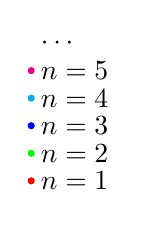
\begin{tikzpicture}[scale=0.5]
            \foreach \n/\c in {1/red,2/green,3/blue,4/cyan,5/magenta}
            {%
                \draw[fill=\c,draw=\c] (0,.7*\n) circle (.5ex) node[right] {$n=\n$};
            }%
            \draw (0,4.2) node[right] {$\cdots$};
        \end{tikzpicture}
    } & 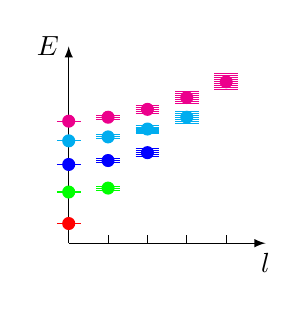
\begin{tikzpicture}[scale=0.5]
        \draw[-latex] (0,0) -- (5,0) node[below] {$l$};
        \draw (1,0) -- (1,0.2);
        \draw (2,0) -- (2,0.2);
        \draw (3,0) -- (3,0.2);
        \draw (4,0) -- (4,0.2);
        \draw[-latex] (0,0) -- (0,5) node[left] {$E$};
        \foreach \n/\c in {1/red,2/green,3/blue,4/cyan,5/magenta}
        {%
            \pgfmathsetmacro\lmax{\n - 1};
            \foreach \l in {0,...,\lmax}%
            {%
                \draw[fill=\c,draw=\c] (\l, {(-0.4+0.95*\n-0.05*\n*\n) + 0.1*\l*(\l+1)/2}) circle (1ex);
                \foreach \m in {-\l,...,\l}%
                {%
                    \draw[\c] (\l - 0.3, {(-0.4+0.95*\n-0.05*\n*\n) + 0.1*\l*(\l+1)/2 + 0.05*\m}) -- (\l + 0.3, {(-0.4+0.95*\n-0.05*\n*\n) + 0.1*\l*(\l+1)/2 + 0.05*\m});
                }%
            }%
        }%
        %
    \end{tikzpicture} & 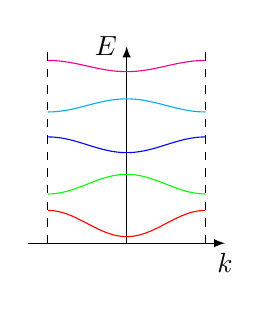
\begin{tikzpicture}[scale=0.5]
        \draw[-latex] (-2.5,0) -- (2.5,0) node[below] {$k$};
        \draw[-latex] (0,0) -- (0,5) node[left] {$E$};
        \draw[dashed] (-2,0) -- (-2,5);
        \draw[dashed] (2,0) -- (2,5);
        \foreach \n/\c in {1/red,2/green,3/blue,4/cyan,5/magenta}
        {%
            \draw[domain=-2:2, smooth, variable=\x, \c] plot ({\x}, {\n-0.5-cos(\x/2*180+180+\n*180)/(\n+2)});
        }%
    \end{tikzpicture} \\
    Symmetry & $\operatorname{SO}(3)$ & $T_N = \mathbb{Z}/(2N\mathbb{Z})$ \\
    Representation & $\rho_{l}: \operatorname{SO}(3)\rightarrow\operatorname{U}(2l+1)$ & $\chi_{k}: T_N \rightarrow \operatorname{U}(1)$ \\
    Label & $l\in\qty{0,1,\cdots}$ & $\displaystyle k\in\qty{\frac{(-N) \pi}{N},\cdots,\frac{(N-1) \pi}{N}}$ \\
    Space & $\mathbb{R}^3$ & $S^1$ \\
    Quotient & $\mathbb{R}^3/\operatorname{SO}(3) = [0,\infty)$ & $S^1/T_N=S^1$ (Unit Cell) \\
    Eigenfunction & $Y_l^m(\theta,\varphi) R_{n,l}(r)$ & $e^{ikR} e^{ikr} u_{n,k}(r)$ \\
    \bottomrule
\end{longtable}

% \bibliographystyle{plain}
% \bibliography{main}

\end{document}
